%% BioMed_Central_Tex_Template_v1.06
%%                   %
% bmc_article.tex      ver: 1.06 %
%                    %

%%IMPORTANT: do not delete the first line of this template
%%It must be present to~enable the BMC Submission system to~
%%recognise this template!!

%%%%%%%%%%%%%%%%%%%%%%%%%%%%%%%%%%%%%%%%%
%%                   %%
%% LaTeX template for BioMed Central %%
%%   journal article submissions   %%
%%                   %%
%%     <14 August 2007>      %%
%%                   %%
%%                   %%
%% Uses:                %%
%% cite.sty, url.sty, bmc_article.cls %%
%% ifthen.sty. multicol.sty		  %%
%%				   	  %%
%%                   %%
%%%%%%%%%%%%%%%%%%%%%%%%%%%%%%%%%%%%%%%%%


%%%%%%%%%%%%%%%%%%%%%%%%%%%%%%%%%%%%%%%%%%%%%%%%%%%%%%%%%%%%%%%%%%%%%
%%                                 %%	
%% For instructions on how to~fill out this Tex template      %%
%% document please refer to~Readme.pdf and the instructions for  %%
%% authors page on the biomed central website           %%
%% http://www.biomedcentral.com/info/authors/           %%
%%                                 %%
%% Please do not use \input{...} to~include other tex files.    %%
%% Submit your LaTeX manuscript as one .tex document.       %%
%%                                 %%
%% All additional figures and files should be attached       %%
%% separately and not embedded in the \TeX\ document its~elf.    %%
%%                                 %%
%% BioMed Central currently use the MikTex distribution of     %%
%% TeX for Windows) of TeX and LaTeX. This is available from   %%
%% http://www.miktex.org                      %%
%%                                 %%
%%%%%%%%%%%%%%%%%%%%%%%%%%%%%%%%%%%%%%%%%%%%%%%%%%%%%%%%%%%%%%%%%%%%%


\NeedsTeXFormat{LaTeX2e}[1995/12/01]
\documentclass[10pt]{bmc_article}  



% Load packages
\usepackage{cite} % Make references as [1-4], not [1,2,3,4]
\usepackage{url} % Formatting web addresses 
\usepackage{ifthen} % Conditional 
\usepackage{multicol}  %Columns
\usepackage[utf8]{inputenc} %unicode support
\usepackage{graphicx}
\usepackage{mathtools}
%\usepackage[applemac]{inputenc} %applemac support if unicode package fails
%\usepackage[latin1]{inputenc} %UNIX support if unicode package fails
\usepackage{color,soul}
\usepackage{amsmath, amssymb}
\usepackage{algorithm2e}
\urlstyle{rm}


\newcommand{\nc}[1]{\begin{flushleft}\hl{[#1]}\end{flushleft}}

 
 
%%%%%%%%%%%%%%%%%%%%%%%%%%%%%%%%%%%%%%%%%%%%%%%%%	
%%                       %%
%% If you wish to~display your graphics for  %%
%% your own use using includegraphic or    %%
%% includegraphics, then comment out the   %%
%% following two lines of code.        %%  
%% NB: These line *must* be included when   %%
%% submitting to~BMC.             %% 
%% All figure files must be submitted as   %%
%% separate graphics through the BMC     %%
%% submission process, not included in the  %% 
%% submitted article.             %% 
%%                       %%
%%%%%%%%%%%%%%%%%%%%%%%%%%%%%%%%%%%%%%%%%%%%%%%%%           


%\def\includegraphic{}
%\def\includegraphics{}



\setlength{\topmargin}{0.0cm}
\setlength{\textheight}{21.5cm}
\setlength{\oddsidemargin}{0cm} 
\setlength{\textwidth}{16.5cm}
\setlength{\columnsep}{0.6cm}

\newboolean{publ}

%%%%%%%%%%%%%%%%%%%%%%%%%%%%%%%%%%%%%%%%%%%%%%%%%%
%%                       %%
%% You may change the following style settings %%
%% Should you wish to~format your article    %%
%% in a~publication style for printing out and %%
%% sharing with colleagues, but ensure that   %%
%% before submitting to~BMC that the style is  %%
%% returned to~the Review style setting.    %%
%%                       %%
%%%%%%%%%%%%%%%%%%%%%%%%%%%%%%%%%%%%%%%%%%%%%%%%%%
 

%Review style settings
%\newenvironment{bmcformat}{\begin{raggedright}\baselineskip20pt\sloppy\setboolean{publ}{false}}{\end{raggedright}\baselineskip20pt\sloppy}

%Publication style settings
%\newenvironment{bmcformat}{\fussy\setboolean{publ}{true}}{\fussy}

%New style setting
\newenvironment{bmcformat}{\baselineskip20pt\sloppy\setboolean{publ}{false}}{\baselineskip20pt\sloppy}


% Begin ...
\begin{document}
\begin{bmcformat}

\newcounter{fig}
\newcounter{pbm}
\newcounter{lm}
\newcounter{def}
\newcounter{rm}


%%%%%%%%%%%%%%%%%%%%%%%%%%%%%%%%%%%%%%%%%%%%%%
%%                                          %%
%% Enter the title of your article here     %%
%%                                          %%
%%%%%%%%%%%%%%%%%%%%%%%%%%%%%%%%%%%%%%%%%%%%%%

\title{Knowledge-based scaling of metabolic models}

%\author{Anna~Zhukova$^1$%
%	\email{Anna~Zhukova - anna.zhukova@inria.fr}%
%and 
%	David~James~Sherman\correspondingauthor$^1$%
%	\email{David~James~Sherman\correspondingauthor - david.sherman@inria.fr}
%}

%\address{%
%\iid(1)INRIA / Universit\'{e} Bordeaux 1 / CNRS joint project-team MAGNOME, Talence, France
%}%

%\maketitle

%%%%%%%%%%%%%%%%%%%%%%%%%%%%%%%%%%%%%%%%%%%%%%
%%                                          %%
%% The Abstract begins here                 %%
%%                                          %%  
%% Please refer to the Instructions for     %%
%% authors on http://www.biomedcentral.com  %%
%% and include the section headings         %%
%% accordingly for your article type.       %%   
%%                                          %%
%%%%%%%%%%%%%%%%%%%%%%%%%%%%%%%%%%%%%%%%%%%%%%






\ifthenelse{\boolean{publ}}{\begin{multicols}{2}}{}




%%%%%%%%%%%%%%%%%%%%%%%%%%%%%%%%%%%%%%%%%%%%%%
%%                                          %%
%% The Main Body begins here                %%
%%                                          %%
%% Please refer to the instructions for     %%
%% authors on:                              %%
%% http://www.biomedcentral.com/info/authors%%
%% and include the section headings         %%
%% accordingly for your article type.       %% 
%%                                          %%
%% See the Results and Discussion section   %%
%% for details on how to create sub-sections%%
%%                                          %%
%% use \cite{...} to cite references        %%
%%  \cite{koon} and                         %%
%%  \cite{oreg,khar,zvai,xjon,schn,pond}    %%
%%  \nocite{smith,marg,hunn,advi,koha,mouse}%%
%%                                          %%
%%%%%%%%%%%%%%%%%%%%%%%%%%%%%%%%%%%%%%%%%%%%%%


%\section*{Abstract}
%Genome-scale metabolic models for new organisms include thousands of reactions that are automatically inferred from databases of reactions and pathways, and from existing models for similar organisms. Genomic data for the new organism is compared to the data of the similar one, to find genomic evidence of the presence of enzymes that can catalyse the conserved reactions in the new model. Starting from the inference of a draft model, the model refinement process includes several iterations of model analysis, error detection, and improvement. The models produced at each iteration are putatively complete, describing all the reactions that participate in the organism's metabolism. These models are intended for computer simulation. Although automatic model inference tools and genome comparison methods are becoming more and more advanced, they still may leave gaps in the model or add erroneous reactions. Thus, model evaluation by human experts remains important at all the iteration steps. However, because of their completeness, genome-scale models are too detailed and complicated to be easily understood by a~human. The abundance of reactions in the model may hide errors.
%
%
%For example, in a model of an yeast \textit{Yarrowia lypolitica}, a missing enzyme \textit{EC 2.3.1.16} would eliminate a whole group of \textit{Acyl-CoA:acetyl-CoA C-acyltransferase} reactions participating in the \textit{Beta-oxidation of fatty acids} pathway: one for each of the six \textit{3-oxoacyl-CoA} species presented in the model. However, the absence of these six reactions may be hidden by the other 59 reactions in the constitutive peroxisome of \textit{Yarrowia lypolitica}, and a human expert may have difficulty noticing the error.
%
%
%We thus developed a~method for knowledge-based zooming of metabolic models, providing a~higher-level view of a~model, keeping its essential structure and omitting the details. The zooming process groups chemical species present in the model into semantically equivalent classes, based on their hierarchical relationships in the ChEBI ontology, and merges them into a generalized chemical species. Reactions that involve same generalized chemical species can then be factored together into a generalized reaction. By applying this process, we can build a simplified model that focusses on the high level relationships. Our method obeys several consistency restrictions, such as conserving the number of distinct species participating in each reaction (i.e. preserving reaction stoichiometry); and not introducing flows between pathways not connected in the initial model. We implemented our method (in Python) and applied it successfully to several genome-scale metabolic models.

%%%%%%%%%%%%%%%%
%% Background %%
%%
\section*{Introduction}
Genome-scale metabolic models for new organisms include thousands of reactions that are automatically inferred from databases of reactions and pathways, and from existing models for similar organisms. Genomic data for the new organism is compared to the data of the similar one, to find genomic evidence of the presence of enzymes that can catalyse the conserved reactions in the new model. Starting from the inference of a draft model, the model refinement process includes several iterations of model analysis, error detection, and improvement~\cite{Thiele2010}. The models produced at each iteration are putatively complete, describing all the reactions that participate in the organism's metabolism. These models are intended for computer simulation. Although automatic model inference tools and genome comparison methods are becoming more and more advanced, they still may leave gaps in the model or add erroneous reactions. Thus, model evaluation by human experts remains important at all the iteration steps. However, because of their completeness, genome-scale models are too detailed and complicated to be easily understood by a~human. The abundance of reactions in the model may hide errors.


For example, in a genome-scale model of an yeast \textit{Yarrowia lypolitica} (\emph{MODEL1111190000}~\cite{Loira12}), a missing enzyme \textit{EC 2.3.1.16} would eliminate a whole group of \textit{Acyl-CoA:acetyl-CoA C-acyltransferase} reactions participating in the \textit{Beta-oxidation of fatty acids} pathway~~\cite{Metzler01}: one for each of the six \textit{3-oxoacyl-CoA} species presented in the model. However, the absence of these six reactions may be hidden by the other 59 reactions in the constitutive peroxisome of \textit{Yarrowia lypolitica}, and a human expert may have difficulty noticing the error.


We thus developed a~method for knowledge-based zooming of metabolic models, providing a~higher-level view of a~model, keeping its essential structure and omitting the details. The zooming process groups chemical species present in the model into semantically equivalent classes, and merges them into a generalized chemical species. Reactions that involve same generalized chemical species can then be factored together into a generalized reaction. By applying this process, we can build a simplified model that focusses on the high level relationships. 

\section*{Mathematical basis}
\subsection*{Basic definitions}
We represent a metabolic model $M$ as a pair of two sets: a set $S$ of biochemical species, and a set $R$ of reactions between them, described in the model: 
\begin{align*} 
& M = \langle S, R \rangle\text{ - model},\\
& S = \{s_1, \ldots, s_n\}\text{ - species set},\\
& R = \{r_1, \ldots, r_m\}\text{ - reaction set}.
\end{align*}
We represent each reaction $r \in R$ as a pair of species sets (a set of its reactant species, and a set of its product species), and a pair of their corresponding stoichiometries. "In a chemical reaction, reactants change into products. A chemical reaction may be represented by a balanced chemical equation, showing the formulae of the reactants and products, and the changes that take place."\cite{Clugston2000} This definition leads to the restriction~(1) that all the species participating in the reaction should be different.
\begin{align} 
\nonumber r = \langle~&\langle\{s^{(react)}_1, \ldots, s^{(react)}_k\},\{s^{(prod)}_1, \ldots, s^{(prod)}_l\}\rangle, \\
\nonumber &\langle\{stoich(s^{(react)}_1), \ldots, stoich(s^{(react)}_k)\},\{stoich(s^{(prod)}_1), \ldots, stoich(s^{(prod)}_l)\rangle~\rangle 
\in \langle\langle 2^S \times 2^S \rangle \times \langle 2^\mathbb{N} \times 2^\mathbb{N} \rangle\rangle , \\
&\text{where }s^{(react)}_1 \neq \ldots \neq s^{(react)}_k \neq s^{(prod)}_1 \neq \ldots \neq s^{(prod)}_l
\end{align}
Further in the text, we will omit the reaction stoichiometry values, for the purposes of simplicity:
\begin{align*} 
r = &\langle\{s^{(react)}_1, \ldots, s^{(react)}_k\},\{s^{(prod)}_1, \ldots, s^{(prod)}_l\}\rangle
\in R \subset \langle 2^S \times 2^S \rangle, \\
&\text{where }s^{(react)}_1 \neq \ldots \neq s^{(react)}_k \neq s^{(prod)}_1 \neq \ldots \neq s^{(prod)}_l
\end{align*}
To generalize the model we will first define an equivalence operation $\sim$ on the species set, and group species into equivalence classes: $[s_i]^{\sim} = \{s_j \in S | s_j \sim s_i\}$.\\
Species equivalence imposes reaction equivalence: two reactions are equivalent if their corresponding reactant and product species are pairwise equivalent.
\begin{center}
$\forall r, \tilde{r} \in R:\; r = \langle\{s^{(react)}_1, \ldots, s^{(react)}_k\},\{s^{(prod)}_1, \ldots, s^{(prod)}_l\}\rangle,$
\end{center}
\begin{center}
$\tilde{r} = \langle\{\tilde{s}^{(react)}_1, \ldots, \tilde{s}^{(react)}_{\tilde{k}}\},\{\tilde{s}^{(prod)}_1, \ldots, \tilde{s}^{(prod)}_{\tilde{l}}\}\rangle$
\end{center}
\begin{align*} 
r \sim \tilde{r} \iff & k = \tilde{k}, l = \tilde{l}, \\
& \forall i\; 0\leq{i}\leq{k} \; \exists \tilde{i}\; 0\leq \tilde{i}\leq \tilde{k}:\; s^{(react)}_i \sim \tilde{s}^{(react)}_{\tilde{i}},\\
& \forall j\;0\leq j\leq l\;\exists \tilde{j}\;0\leq \tilde{j}\leq\tilde{l}:\;s^{(prod)}_j \sim \tilde{s}^{(prod)}_{\tilde{j}}.
\end{align*}
Generalized reactions (i.e. reaction equivalence classes) thus operate with generalized species (i.e. species equivalence classes): 
$[r]^{\sim} = \langle\{[s^{(react)}_1]^{\sim}, \ldots, [s^{(react)}_k]^{\sim}\}, \{[s^{(prod)}_1]^{\sim}, \ldots, [s^{(prod)}_l]^{\sim}\}\rangle$.\\
Note, that in order to keep the number of distinct species participating in a reaction (preserve its stoichiometry) the restriction~(2), analogous to the restriction~(1), should be satisfied:
\begin{align}
[s^{(react)}_1]^{\sim} \neq \ldots \neq [s^{(react)}_k]^{\sim} \neq [s^{(prod)}_1]^{\sim} \neq \ldots \neq [s^{(prod)}_l]^{\sim}
\end{align}
Thus the generalized model $M/\sim$ is a pair of generalized species and reaction sets (quotient sets):
\begin{align*} 
&M/\sim = \langle S/\sim, R/\sim \rangle\text{ - generalized model},\\
&S/\sim = \{[s_1]^{\sim}, \ldots, [s_{\tilde{n}}]^{\sim}\}\text{ - quotient species set},\\
&R/\sim = \{[r_1]^{\sim}, \ldots, [r_{\tilde{m}}]^{\sim}\}\text{ - quotient reaction set}.
\end{align*}
%\subsection*{Restriction 2}
%In order for the generalization process not to introduce connections between pathways disconnected in the initial model, we add a restriction that for each indirected path between two reactions in the generalized model, there should exist a prototype path in the initial model.
%$\forall [s] \in S/\sim (\exists [r_1], [r_2] \in R/\sim: [s] \in species([r_1]) \cap species([r_2]) \implies \exists s \in S, \exists r_1, r_2 \in R: s \in [s], r_1 \in [r_1], r_2 \in [r_2], s \in species(r_1) \cap species(r_2))$

\subsection*{Ubiquitous species}
The species in the model are divided into two groups: ubiquitous and specific. Ubiquitous species are those participating in most of the reactions, such as water, hydrogen, oxygen, etc. They are common for most of the models, thus do not need to be generalized. In the generalized model each of them forms a one-element equivalence class:
\begin{align*}
S^{(ub)} = \{s^{(ub)}_1, \ldots, s^{(ub)}_{\breve{n}}\} \subset S: \forall i\,[s^{(ub)}_i]^{\sim} = \{s^{ub}_i\}
\end{align*}
 Specific species are all the others, they are divided into equivalence classes and generalized accordingly.  

\newtheorem{p0}[pbm]{Problem}
\begin{p0}
Given a metabolic model $M=\langle S, S^{(ub)} \subset S, R \rangle$ that describes $n$ species (including $\breve{n} \leq n$ ubiquitous ones) and $m$ reactions, find an equivalence operation $\sim$ that obeys the restriction~(2), and minimizes the number of reaction equivalence classes $\sharp R/\sim$. Among such equivalence operations choose the one that defines the maximal number of species equivalence classes $\sharp S/\sim$, i.e., generalize as many reactions as possible, while keeping species maximally specific.
\end{p0}
\newtheorem{eq0}[def]{Definition}
\begin{eq0}
Given a model $M=\langle S, S^{(ub)}\subset{S}, R \rangle : \sharp S = n, \sharp S^{(ub)}=\breve{n} \leq n, \sharp R = m$, let us define an equivalence operation $\mathring{\sim}$ on the species set $S$ as one, forming $\breve{n} + 1$ equivalence classes in the quotient set $S/\mathring{\sim}$: one for each of the ubiquitous species, and one for all the other species:
\begin{align*}
&\forall s^{(ub)} \in S^{(ub)} \;[s^{(ub)}]^{\mathring{\sim}} = \{s^{(ub)}\}, \\
&\forall s, \tilde{s} \in S\backslash S^{(ub)} \;[s]^{\mathring{\sim} } = [\tilde{s}]^{\mathring{\sim} } = S \backslash S^{(ub)}.
\end{align*}
\end{eq0}
\newtheorem{l1}[lm]{Lemma}
\begin{l1}
For any equivalence operation $\sim$ on the model $M=\langle S, S^{(ub)} \subset S, R \rangle$, the quotient species set $S/\sim$ and the quotient reaction set $R/\sim$ induced by $\sim$ are partitions of respectively the quotient species set $S/\mathring{\sim}$ and the quotient reaction set $R/\mathring{\sim} $ induced by $\mathring{\sim}$:
\begin{align*}
\forall \sim &\text{ defined on }\langle S, S^{(ub)}, R \rangle\\
&\forall s \in S \; [s]^{\sim} \subset [s]^{\mathring{\sim}} \\
&\forall r \in R \; [r]^{\sim} \subset [r]^{\mathring{\sim}} 
\end{align*}
\end{l1}

\begin{algorithm}[H]
\SetAlgoVlined
\TitleOfAlgo{Compute$\mathring{\sim}$}
\caption{Computation of $\mathring{\sim}$}
\KwData{$M=\langle{S, S^{(ub)}\subset{S}, R}\rangle: \sharp S = n, \sharp S^{(ub)}=\breve{n} \leq n, \sharp R = m$ - metabolic model describing $n$ species,  $\breve{n}$ among them being ubiquitous,  and $m$ reactions.}
\KwResult{$\mathring{\sim}$ - equivalence operation described in Lemma~1, $M/{\mathring{\sim}} = \langle S/{\mathring{\sim}}, S^{(ub)}/{\mathring{\sim}} \subset S/{\mathring{\sim}}, R/{\mathring{\sim}} \rangle$ - corresponding generalized model.}
\BlankLine
\BlankLine
$S/{\mathring{\sim}} \leftarrow \emptyset$ \tcp*[l]{resultant quotient species set $ S/{\mathring{\sim}}\subset 2^S$}
$S^{(ub)}/{\mathring{\sim}} \leftarrow \emptyset$ \tcp*[l]{resultant quotient ubiquitous species set $ S^{(ub)}/{\mathring{\sim}}\subset 2^{S^{(ub)}}$}
$R/{\mathring{\sim}} \leftarrow \emptyset$ \tcp*[l]{resultant quotient reaction set $ R/{\mathring{\sim}}\subset 2^R$}
$\mathring{\sim} \leftarrow \emptyset$ \tcp*[l]{resultant equivalence operation $ {\mathring{\sim}}: S\cup{R} \rightarrow S/{\mathring{\sim}}\cup{R/{\mathring{\sim}}}$}
\BlankLine
\BlankLine
\tcc{Generalize ubiquitous species}
\For {$s^{(ub)} \in S^{(ub)}$} {
	$\mathring{\sim}(s^{(ub)}) \leftarrow \{s^{(ub)}\}$ \;
}
$S^{(ub)}/{\mathring{\sim}} \leftarrow \{\{s^{(ub)}\}|s^{(ub)} \in S^{(ub)}\}$ \;
\BlankLine
\BlankLine
\tcc{Generalize non-ubiquitous species}
\For {$s \in S \backslash S^{(ub)}$} {
	$\mathring{\sim}(s)  \leftarrow S \backslash S^{(ub)}$ \;
}
$S/{\mathring{\sim}} \leftarrow {S^{(ub)}/{\mathring{\sim}}}\cup\{S \backslash S^{(ub)}\}$ \;
\BlankLine
\BlankLine
\tcc{Generalize reactions}
\BlankLine
\tcp{map a reaction to its generalized version that operates with generalized species}
$gen \leftarrow \lambda{r}.\langle\mathring{\sim}(reactants(r)), \mathring{\sim}(products(r))\rangle$ \;
\BlankLine
\For {$r \in R$} {
	$\mathring{\sim}(r) \leftarrow \{\tilde{r} \in R|gen(\tilde{r})=gen(r)\}$ \;
}
$R/{\mathring{\sim}} \leftarrow \{\mathring{\sim}(r)|r \in R\}$ \;
\BlankLine
\KwRet{$\mathring{\sim}, \langle S/{\mathring{\sim}}, S^{(ub)}/{\mathring{\sim}}, R/{\mathring{\sim}} \rangle$}
\end{algorithm} 

\subsection*{Species equivalence class number maximization}
\newtheorem{p1}[pbm]{Problem}
\begin{p1}
Given an equivalence operation $\sim$ defined on a metabolic model $M=\langle S, S^{(ub)}\subset{S}, R \rangle$, such that $\sim$ obeys the restriction~(2), find an equivalence operation $\tilde{\sim}$ that does not change the reaction equivalence classes: $R/\sim = R/\tilde{\sim}$, and maximizes the number of species equivalence classes $\sharp S/\tilde{\sim}$. 
\end{p1}
%To find an equivalence operation $\sim$ satisfying the restrictions described above, we will start with the operation  $\mathring{\sim}$ as the first approximation and continue improving it till all the restrictions are satisfied. 

%%First of all, we will satisfy the restriction 2 for each pair of reactions violating it: \\
%%$\forall [r_i]_{\approx}, [r_j]_{\approx} \in R/\approx: [s]_{\approx} \in species([r_i]) \cap species([r_j]),  \forall r_i \in [r_i]_{\approx} \forall r_j \in [r_j]_{\approx}:  species(r_i) \cap species(r_j) \subset S^{(ub)}$. \\
%First of all, we will maximize the number of species equivalence classes for the equivalence operation $\mathring{\sim}$.
\subsubsection*{Algorithm}
To maximize the number of species equivalence classes for the equivalence operation $\tilde{\sim}$ we will associate each species $s$ in the initial model to a pair of reaction equivalence classes sets in the quotient reaction set $R/{\sim}$: those induced by reactions where it participates as a reactant, and as a product: $s \rightarrow \langle R^{(react)}_s = \{[r^{(react)}_1]^{\sim}, \ldots, [r^{(react)}_o]^{\sim}\}, R^{(prod)}_s = \{[r^{(prod)}_1]^{\sim}, \ldots, [r^{(prod)}_t]^{\sim}\}\rangle$.

We will define the equivalence operation $\tilde{\sim}$ as forming a separate species equivalence class for each of the ubiquitous species, and putting $\sim$-equivalent non-ubiquitous species that intersect in their product or reactant reaction classes in the same equivalence class:
\begin{alignat*}{3}
& \forall s^{(ub)} \in S^{(ub)}, s \in S \;\; & s^{(ub)} \tilde{\sim} s \iff & s^{(ub)} = s, \\
& \forall s, \tilde{s} \in S \backslash S^{(ub)} \; & s \tilde{\sim} \tilde{s} \iff 
& s \sim \tilde{s}\;\land & (R^{(react)}_s \cap R^{(react)}_{\tilde{s}} \neq \emptyset\\
& ~ &  ~ &~ &\lor R^{(prod)}_s \cap R^{(prod)}_{\tilde{s}} \neq \emptyset\\
& ~ &  ~ &~ &\lor \exists \dot{s} \in S:\; s \tilde{\sim} \dot{s} \land \tilde{s} \tilde{\sim} \dot{s}). 
\end{alignat*}
Any further partition of the quotient species set would imply the partition of the quotient reaction set. Hence the number of species equivalence classes is maximal for the current number of reaction equivalence classes. \\

\begin{algorithm}[H]
\SetAlgoVlined
\TitleOfAlgo{Maximize}
\caption{Maximization of the Number of Species Equivalence Classes}
\KwData{${\sim}$ - equivalence operation defined on a metabolic model $M=\langle S, S^{(ub)}\subset{S}, R \rangle$, $M/{\sim} = \langle S/{\sim}, S^{(ub)}/{\sim} \subset S/{\sim}, R/{\sim} \rangle$ - corresponding generalized model.}
\KwResult{$\tilde{\sim}$ - equivalence operation described in Problem~2, $M/\tilde{\sim} = \langle S/\tilde{\sim}, S^{(ub)}/\tilde{\sim} \subset S/\tilde{\sim}, R/\tilde{\sim} \rangle$ - corresponding generalized model.}
\BlankLine
\BlankLine
$S/\tilde{\sim} \leftarrow \emptyset$ \tcp*[l]{resultant quotient species set $ S/{\tilde{\sim}}\subset 2^S$}
$S^{(ub)}/\tilde{\sim} \leftarrow S^{(ub)}/\sim$ \tcp*[l]{resultant quotient ubiquitous species set $ S^{(ub)}/{\tilde{\sim}}\subset 2^{S^{(ub)}}$}
$R/\tilde{\sim} \leftarrow R/\sim$ \tcp*[l]{resultant quotient reaction set $ R/{\tilde{\sim}}\subset 2^R$}
$\tilde{\sim} \leftarrow \sim$ \tcp*[l]{resultant equivalence operation $ {\tilde{\sim}}: S\cup{R} \rightarrow S/{\tilde{\sim}}\cup{R/{\tilde{\sim}}}$}
\BlankLine
\BlankLine
\tcc{Update non-ubiquitous species generalization}
\BlankLine
\tcp{Map a species to a set of its $\sim$-equivalent species}
\tcp{that participate in $\sim$-equivalent reactions}
$r\_sim \leftarrow \lambda{s}.\{\tilde{s}\in\sim(s)|\exists r,\tilde{r}\in{R}: s\in reactants(r) \land \tilde{s}\in reactants(\tilde{r}) \land r \sim \tilde{r}\}$ \;
$p\_sim \leftarrow \lambda{s}.\{\tilde{s}\in\sim(s)|\exists r,\tilde{r}\in{R}: s\in products(r) \land \tilde{s}\in products(\tilde{r}) \land r \sim \tilde{r}\}$ \;
$sim \leftarrow \lambda{s}.r\_sim(s)\cup p\_sim(s)$ \;
\BlankLine
$S/\tilde{\sim} \leftarrow S^{(ub)}/\tilde{\sim} \cup \{sim(s)|s \in S\backslash S^{(ub)}\}$ \;
\BlankLine
\tcp{Merge all quotient species sets that intersect}
\While {$\exists S^{(gen)} \neq \tilde{S}^{(gen)} \in S/\tilde{\sim}: S^{(gen)} \cap \tilde{S}^{(gen)} \neq \emptyset$} {
	$S/\tilde{\sim} \leftarrow (S/\tilde{\sim}\backslash{\{S^{(gen)}, \tilde{S}^{(gen)}\}})\cup\{S^{(gen)}\cup \tilde{S}^{(gen)}\}$ \;
}
\BlankLine
\tcp{Update $\tilde{\sim}$}
\For {$S^{(gen)}\in{S/\tilde{\sim}}$} {
	\For {$s \in S^{(gen)}$} {
		$\tilde{\sim}(s) = S^{(gen)}$ \;
	}
}
\BlankLine
\KwRet{$\tilde{\sim}, \langle S/\tilde{\sim}, S^{(ub)}/\tilde{\sim}, R/\tilde{\sim} \rangle$}
\end{algorithm} 

\subsection*{Stoichiometry preserving property obedience}
\newtheorem{p2}[pbm]{Problem}
\begin{p2}
Given an equivalence operation $\sim$ defined on a metabolic model $M=\langle S, S^{(ub)}\subset{S}, R \rangle$ find an equivalence operation $\tilde{\sim}$ that obeys the stoichiometry preserving property~(2) and induces a quotient species set $S/\tilde{\sim}$ of minimal size $\sharp S/\tilde{\sim}$, such that $S/\tilde{\sim}$ is a partition of the quotient species set $S/\sim$ induced by $\sim$, i.e., $\forall s \in S \; [s]^{\tilde{\sim}} \subset [s]^{\sim} $. 
\end{p2}
\subsubsection*{Algorithm}
We will start with the given equivalence operation $\sim^0 = \sim$, and iteratively improve it, until the stoichiometry preserving property~(2) is obeyed. We will denote the equivalence operation obtained at the $i$-th iteration step as $\sim^i$.

At each iteration, if there exists a species equivalence class that violates the stoichiometry preserving property~(2), i.e.:
\begin{align*}
\exists s \neq \tilde{s} \in S, r \in R: s \in species(r) \land \tilde{s} \in species(r) \land  [s]^{{\sim}^i} = [\tilde{s}]^{{\sim}^i},
\end{align*}
we will partition this species equivalence class $[s]^{{\sim}^i} = [\tilde{s}]^{{\sim}^i}$ into two: $[s]^{{\sim}^{i+1}}  \vee [\tilde{s}]^{{\sim}^{i+1}}  = [s]^{{\sim}^i} = [\tilde{s}]^{{\sim}^i} $ to form a new approximation ${\sim}^{i+1}$ of the equivalence operation. When no species equivalence class violating the stoichiometry preserving property~(2) can be found, the current equivalence operation is returned as result.

As at each iteration one equivalence species class is partitioned, and the equality operation $=$ (each species is equivalent only to itself), that will be achieved in the worst case, obeys the stoichiometry preserving property~(2), so the process will terminate. \\


\begin{algorithm}[H]
\SetAlgoVlined
\TitleOfAlgo{PreserveStoichiometry}
\caption{Stoichiometry Preserving Property Obedience}
\KwData{${\sim}$ - equivalence operation defined on a metabolic model $M=\langle S, S^{(ub)}\subset{S}, R \rangle$, $M/{\sim} = \langle S/{\sim}, S^{(ub)}/{\sim} \subset S/{\sim}, R/{\sim} \rangle$ - corresponding generalized model.}
\KwResult{$\tilde{\sim}$ - equivalence operation described in Problem~3, $M/\tilde{\sim} = \langle S/\tilde{\sim}, S^{(ub)}/\tilde{\sim} \subset S/\tilde{\sim}, R/\tilde{\sim} \rangle$ - corresponding generalized model.}
\BlankLine
\BlankLine
$S/\tilde{\sim} \leftarrow S/\sim$ \tcp*[l]{resultant quotient species set $ S/{\tilde{\sim}}\subset 2^S$}
$S^{(ub)}/\tilde{\sim} \leftarrow S^{(ub)}/\sim$ \tcp*[l]{resultant quotient ubiquitous species set $ S^{(ub)}/{\tilde{\sim}}\subset 2^{S^{(ub)}}$}
$R/\tilde{\sim} \leftarrow \emptyset$ \tcp*[l]{resultant quotient reaction set $ R/{\tilde{\sim}}\subset 2^R$}
$\tilde{\sim} \leftarrow \sim$ \tcp*[l]{resultant equivalence operation $ {\tilde{\sim}}: S\cup{R} \rightarrow S/{\tilde{\sim}}\cup{R/{\tilde{\sim}}}$}
\BlankLine
\BlankLine
\tcc{Partition quotient species that do not obey the stoichiometry preserving property~(2)}
\For {$S^{(gen)} \in \{\tilde{S}^{(gen)}\in S/\tilde{\sim}| \exists s \neq \tilde{s} \in \tilde{S}^{(gen)}, r \in R:  s \in species(r) \land \tilde{s} \in species(r)\}$}{
	$\Phi = Partition(S^{(gen)})$ \;
	\BlankLine
	\tcp{Update $S/\tilde{\sim}$}
	$S/\tilde{\sim} \leftarrow S/\tilde{\sim}\cup\Phi$ \;
	\BlankLine
	\tcp{Update $\tilde{\sim}$}
	\For {$\tilde{S}^{(gen)} \in \Phi$} {
		\For {$s \in \tilde{S}^{(gen)}$} {
			$\tilde{\sim}(s) = \tilde{S}^{(gen)}$ \;
		}
	}
}
\BlankLine
\BlankLine
\tcc{Generalize reactions}
\BlankLine
\tcp{map a reaction to its generalized version that operates with generalized species}
$gen \leftarrow \lambda{r}.\langle\tilde{\sim}(reactants(r)), \tilde{\sim}(products(r))\rangle$ \;
\BlankLine
\For {$r \in R$} {
	$\tilde{\sim}(r) \leftarrow \{\tilde{r} \in R|gen(\tilde{r})=gen(r)\}$ \;
}
$R/{\tilde{\sim}} \leftarrow \{\tilde{\sim}(r)|r \in R\}$ \;
\BlankLine
\KwRet{$\tilde{\sim}, \langle S/\tilde{\sim}, S^{(ub)}/\tilde{\sim}, R/\tilde{\sim} \rangle$}
\end{algorithm} 

We will now describe the species equivalence class partition.

\subsubsection*{Clique partition}
\newtheorem{scg}[def]{Definition}
\begin{scg}
Species compatibility graph is a simple undirected graph corresponding to a species equivalence class. It represents all the species as vertices. For each pair of species that do not participate in the same reaction (i.e., putting them into the same equivalence class does not violate the stoichiometry preserving property~(2)) there exists an edge between them in the species compatibility graph. There are no other edges in the species compatibility graph.
\end{scg}
Note, that any set of species that can be put into the same equivalence class without violating the stoichiometry preserving property~(2), forms a clique  in the species compatibility graph, i.e. a complete subgraph: for every pair of its vertices there exists an edge linking them. Thus, the problem of partition the species equivalence class into minimum number of classes, such that all of them obey the stoichiometry preserving property~(2) is a clique partition problem.
\newtheorem{clp}[pbm]{Problem}
\begin{clp}[Clique partition]
Find the smallest number of cliques in a graph such that every vertex in the graph is represented in exactly one clique.
\end{clp}
\newtheorem{rem0}[rm]{Remark}
\begin{rem0}
Clique partition problem is known to be \textit{NP}-complete~\cite{Bhasker1991}. 
\end{rem0}

%In such kind of a graph produced from a metabolic model there are usually few edges missing, often not more, than one edge per species. When this is the case, multiple solutions of the size 2 are possible, e.g. obtained by splitting all the "problematic" nodes (missing one edge) into two cliques, such that for each of these nodes its partner node (the one to which the missing edge would connect) is placed into the other clique. Each of the rest of the nodes ("non-problematic" ones, i.e. having the maximal edge degree) can be placed into any of the cliques. The choice of the clique for each of the "non-problematic" nodes leads to different solutions. I.e. the complement (inverse) of the graph G  is bipartite.

\subsubsection*{Species ontology}
In a species compatibility graph, there are usually few edges missing, and multiple solutions of the clique partition problem exist. In order to make the choice of the species equivalence classes biologically meaningful, we will use an ontology that describes hierarchical \textit{is\_a} relationships (i.e. more specific - more general) between biochemical species. This ontology can be viewed as a directed acyclic graph, with nodes representing terms describing species, and edges representing hierarchical relationships between them. A term $T$ is an ancestor of a term $t$ if and only if there exists a path from $t$ to $T$. 

\newtheorem{mt}[def]{Definition}
\begin{mt}
A term $t$ is a model term if it corresponds to a non-ubiquitous species in the metabolic model. 
\end{mt}
We will assume that no two model terms are connected by a descendant-ancestor relationship in the ontology (Otherwise, we will mark the ancestor term ubiquitous): $\forall t, T \in terms \; (\exists\, species(t), species(T) \in S \land t \in descendants(T) \implies t = T)$.

We will iteratively remove all the leaf terms that are not model terms from the ontology, so that all the model terms become leaves, and all the leaves become model terms. 

For each species equivalence class that needs to be partitioned, we will first find the least common ancestor $T$ of the ontological terms corresponding to its species. If the ontology allows for multiple inheritance, and there are several such least common ancestors, we will pick the first one. Then we will look among $T$-th descendant terms for those that are compatible (to avoid multiple inheritance).

\newtheorem{comp}[def]{Definition}
\begin{comp}
Terms $ t_1, \ldots, t_k$ are compatible if and only if their descendant model terms do not intersect:
$ t_1, \ldots, t_k \in descendants(T) \text{ are compatible} \iff \forall i \neq j \in \{1, \ldots, k\} \; descendants(t_i) \cap descendants(t_k) \cap leaves(T) = \emptyset$.
\end{comp}

\newtheorem{pp}[pbm]{Problem}
\begin{pp}
Given a term $T$, find a compatible term set of minimal size that covers all the $T$-th descendant leaf terms and satisfies the stoichiometry preserving property~(5):
\begin{align}
\nonumber ?\; t_1, \ldots, t_k \in descendants(T):\; & k = k_{min},\\
&t_1, \ldots, t_k \text{ are compatible},\\
&leaves(T) \subset descendants(t_1) \cup \ldots \cup descendants(t_k) ,\\
&\forall i \neq j \in \{1, \ldots, k\}\; (\exists\, species(t_i), species(t_j) \in S \implies \\
\nonumber &\indent \forall r \in R: \{species(t_i), species(t_j)\} \not \subset species(r)).
\end{align}
\end{pp}
To do so, we will first exclude all the terms that violate the stoichiometry preserving property~(5). We thus obtain an exact set cover problem. 

\newtheorem{setc}[pbm]{Problem}
\begin{setc}[Set cover]
An instance consists of a set $X$ and a collection of its finite subsets $\Psi$, such that $\bigcup_{S \in \Psi} S = X$. We say that a subset $S$ covers its own elements. The problem is to find a minimum-size subset $\Phi \subset \Psi$ whose members cover all of $X$: $\bigcup_{S \in \Phi} S = \bigcup_{S \in \Psi} S = X$.
\end{setc}
\newtheorem{rem}[rm]{Remark}
\begin{rem}
 Set cover is \textit{NP}-complete~\cite{Cormen2001}.
\end{rem}

\newtheorem{esetc}[pbm]{Problem}
\begin{esetc}[Exact set cover]
The exact cover problem is similar to the set cover problem, except that here the sets that are used in the cover are not allowed to intersect. 
\end{esetc}
\newtheorem{rem1}[rm]{Remark}
\begin{rem1}
Exact cover is \textit{NP}-complete~\cite{Goldreich2008}.
\end{rem1}

\subsubsection*{Our case}
Each ontological term $t$ defines a set $S(t)$ of its descendant (including $t$ if it is a leaf) leaf terms. The instance consists of a set $X$ of all leaf descendants of the least common ancestor $T$ of the model terms of interest, and a collection $\Psi$ of all sets defined by $T$-th descendant terms, and their relative complements with respect to $X$: $\forall S \in \Psi \; X\backslash S \in \Psi$, excluding all the sets that violate the stoichiometry preserving property~(5). We look for a minimum-size exact cover of $X$. 

Note, that in our case an exact cover always exists, e.g. the one formed by all the leaf terms.

\subsubsection*{Choice of the ontology}
We will assume that all the terms that violate the stoichiometry preserving property~(5) are removed from the ontology. Note, that the term $T$ will be also removed.

%by removing every such term, and moving its child terms one level up in the hierarchy, so that they become child terms of each of its parent terms. From the graph point of view, it means that for each removed vertex (corresponding to an eliminated term) an edge is added between every source vertex of its input edges and every target vertex of its output edges. 

If the ontology has no multiple inheritance, i.e. $\forall S, \tilde{S} \in \Psi \; S \cap \tilde{S} \neq \emptyset \implies S \subseteq \tilde{S} \lor \tilde{S} \subseteq S$, the problem becomes trivial: The set of the root terms forms the solution. The size of the solution though depends on the characteristics of the ontology, e.g. for a completely flat ontology (i.e., a graph with no edges) the solution will consist of singleton equivalence classes.

If the multiple inheritance is allowed, any $\Psi \subseteq 2^X$ becomes possible, and the problem becomes \textit{NP}-complete. 

We will use the ChEBI ontology~\cite{deMatos10}, which classifies chemical compounds, and is \textit{de facto} a standard for species annotation in metabolic models. ChEBI consists of three main branches: \textit{chemical entity}, \textit{role}, and \textit{subatomic particle}. The \textit{chemical entity} branch describes terms useful for annotation of biochemical species in a metabolic model. As of ChEBI version 101, this branch contains 37693 terms, among which 29888 are leaves. ChEBI has multiple inheritance with average number of parents 1.4 per term. Average number of siblings is also 1.4 per term. Maximal depth in the \textit{chemical entity} branch is 28, while the average one is 11.

The level of details in the ChEBI hierarchy is not uniform: some sub-branches are more developed than others, which makes equally specific terms to be placed unequally deep in the hierarchical tree. For example, both \textit{hydrogen peroxide (CHEBI:16240)} and \textit{decanoyl-CoA (CHEBI:28493)} terms describe precise chemical molecules; but \textit{hydrogen peroxide} is only 5 terms away from the \textit{chemical entity} in the ChEBI hierarchy, while \textit{decanoyl-CoA} is 11 terms away. 

Besides that, different types of classification are combined together in the hierarchical tree, leading to multiple inheritance. For example, in the \textit{fatty-acid (CHEBI:35366)} sub-branch, several types of the classification are present, including
\begin{itemize}
\item classification based on the length of the carbon chain:
\begin{itemize}
\item \textit{short-chain fatty acid (CHEBI:26666)}: 2-4 carbons;
\item \textit{medium-chain fatty acid (CHEBI:59554)}: 6-12 carbons;
\item \textit{long-chain fatty acid (CHEBI:15904)}: 14-22 carbons;
\item \textit{very long-chain fatty acid (CHEBI:27283)}: 24 -26 carbons;
\end{itemize}
\item classification based on the presence of double bonds in the carbon chain:
\begin{itemize}
\item \textit{saturated fatty acid (CHEBI:26607)}: no double bonds;
\item \textit{unsaturated fatty acid (CHEBI:27208)}: one or more double bonds.
\end{itemize}
\end{itemize}

Moreover, it turns out that using only hierarchical relationships on the ChEBI ontology is not always enough. Examples show, that similar reactions can happen to the acid and the base in a conjugate acid-base pair. A conjugate acid-base pair is two species, one an acid and one a base, that differ from each other through the loss or gain of a proton~\cite{stoker2012general}. For instance, in the Rhea database of chemical reactions~\cite{Alcantara2012}, the \textit{acyl-CoA oxidase (RHEA:28354)} reaction: $\textit{decanoyl-CoA} + \textit{FAD} + \textit{H+} \rightarrow \textit{trans-dec-2-enoyl-CoA} + $\textit{FADH$_2$} is found for both \textit{decanoyl-CoA~(CHEBI:28493)} and its conjugate base \textit{decanoyl-CoA(4-)~(CHEBI:61430)}. But hierarchically, these species are very far from each other in the ChEBI ontology: The least common ancestor of \textit{decanoyl-CoA} and \textit{decanoyl-CoA(4-)} is \textit{molecular entity (CHEBI:23367)}, a direct child of the root \textit{chemical entity}. To establish a conjugate acid-base pair correspondence in the ChEBI ontology not the hierarchical (\textit{is\_a}) but special \textit{is\_conjugate\_base\_of} and \textit{is\_conjugate\_acid\_of} relationships, being inverse of each other, are used. To maximize the chances of a conjugate acid-base pair being in the same quotient species set, we will generalize the hierarchical relationship:

\newtheorem{dirgent}[def]{Definition}
\begin{dirgent}
Term $t$ is a generalized direct descendant/ancestor of a term $T$ if and only if $t$ or a conjugate base/acid of $t$ is a direct descendant/ancestor of $T$ or of a conjugate base/acid of $T$.
\end{dirgent} 

\newtheorem{gent}[def]{Definition}
\begin{gent}
Term $t$ is a generalized descendant/ancestor of a term $T$ if and only if $t$ is a generalized direct descendant/ancestor of $T$ or of any generalized descendant/ancestor of $T$.
\end{gent} 



We will extend $Psi$ so that it has closure under the operation of relative complement: $\forall S,\tilde{S} \in \Psi \; S\backslash\tilde{S} \in \Psi$. This will allow for solving the set cover problem instead of the exact cover one:  As $Psi$ has closure under the operation of complement intersection, we can obtain an exact set cover $\tilde{C}$ from any set cover $C = \{S_1, S_2, \ldots, S_m\}$ by replacing its elements with their relative complements with the previous elements of $C$: $\tilde{C} = \{S_1, S_2 \backslash S_1, \ldots, S_m \backslash \bigcup^{m - 1}_{i = 1}{S_i}\}$.

%Notice, that following two statements are True for a sub-branch ($X$, $\Psi$, $T$) of the \textit{chemical entity} branch induced by any term $T$:
%\begin{enumerate}
%\item We can produce an exact cover $\Phi^{(Y)} \subset \Psi$ of any $Y \subset X$ by forming it from all the one-element sets for each of the elements of $Y$: $\Phi^{(Y)} = \{\{x\}| \forall x \in Y\}$. This cover contains the maximal number of elements among all the possible exact covers of $Y$.
%\item Given any subset $\Theta$ of $\Psi$ such that all the elements of $\Theta$ are pairwise disjoint: $\forall S, \tilde{S} \in \Theta \; S \cap \tilde{S} = \emptyset$, a union of $\Theta$ and an exact cover $\Phi^{(X \backslash \bigcup_{S \in \Theta} S)}$ of $X \backslash \bigcup_{S \in \Theta} S$ will form an exact cover of $X$: $\Phi^{(X)} = \Theta \cup \Phi^{(X \backslash \bigcup_{S \in \Theta} S)}$
%
%\item For any set $S$ that includes all the sets it intersects with: $\tilde{S} \in \Psi \; S \cap \tilde{S} \neq \emptyset \implies \tilde{S} \subset S$ (i.e. it is a root term and all the ancestors of any of its descendants are also descendants of $T$: $S \text{ is a root and } ancestors(descendants(T)) \subset descendants(T)$), it is included in the minimal exact cover $\Phi^{(X)}_{min}$ of $X$.
%\item For any set $S$ that belongs to an exact cover $\Phi^{(X)}$ of $X$, any set $\tilde{S} \in \Psi \backslash \{S\}$ that intersects with $S$ does not belong to $\Phi^{(X)}$.
%\end{enumerate}
%
%We will introduce an algorithm of finding the minimal exact cover, based on these statements.
%\begin{algorithm}[H]
%\SetAlgoVlined
%\TitleOfAlgo{minCover}
%\caption{minCover}
%\LinesNumbered
%\KwData{$X$ - the set of interest, $\Psi$ - set of subsets of $X$, $min\_cover\_size \leftarrow \sharp X$ - initial minimal cover size}
%\KwResult{$C$ - minimal exact cover of $X$}
%\BlankLine
%%def minCover(\(X, \Psi, min\_cover\_size\))
%$\Psi \leftarrow \Psi\backslash\{\{x\}|x\in{X}\}$ \tcp*[l]{remove one-element subsets from $\Psi$}
%$C \leftarrow \emptyset$ \tcp*[l]{a set to contain the result}
%\BlankLine
%\For (\tcc{According to the statement~3, add all the sets that include all the sets they intersects with, to the exact cover $C$}) {$S \in \{\dot{S} \in \Psi | \forall \tilde{S} \in \Psi \backslash \{\dot{S}\}  \; \tilde{S} \cap \dot{S} \neq \emptyset \implies \tilde{S} \subset \dot{S}\}$}{
%$C \leftarrow C \cup \{S\}$ \tcp*[l]{according to the statement~3}
%$\Psi \leftarrow \Psi \backslash \{\tilde{S} \in \Psi| \tilde{S} \cap S \neq \emptyset\}$ \tcp*[l]{according to the statement~4}
%$X \leftarrow X \backslash S$ \tcp*[l]{according to the statement~2}
%$min\_cover\_size \leftarrow min\_cover\_size - 1$ \;
%}
%\BlankLine
%\eIf (\tcc{According to the statement~1, there always exists an exact cover composed of one-element subsets of $X$ }) {$\Psi = \emptyset$}{
%	\eIf{$\sharp{X} < min\_cover\_size$}{
%		$min\_cover\_size \leftarrow \sharp{X}$ \;
%		return $C \cup \{\{x\} | x \in X\}$ \;
%	}{
%		return $None$ \;
%	}
%\BlankLine
%}  ( \tcc{For each element of $\Psi$, calculate the minimal exact cover, that includes it; and select the minimal among those exact covers}) {
%	$\Theta \leftarrow sorted(\Psi, criterion=\lambda{S\tilde{S}}.\sharp{S}<\sharp\tilde{S})$ \tcp*[l]{sets sorted by their size, in the descendent order}
%	$\Gamma \leftarrow \emptyset$ \tcp*[l]{possible exact covers}
%	\For {$S \in \Theta$}{
%		$\tilde{C} \leftarrow minCover(X \backslash S, \Psi \backslash \{\tilde{S} \in \Psi| \tilde{S} \cap S \neq \emptyset\}, min\_cover\_size -1)$ \;
%		\If{$\tilde{C} \neq None \land \sharp{\tilde{C}} + 1 < min\_cover\_size$}{
%			$min\_cover\_size \leftarrow \sharp{\tilde{C}} + 1$ \;
%			$\Gamma \leftarrow \Gamma \cup \{\{S\} \cup \tilde{C}\}$ \;
%		}
%	}	
%	\eIf{$\Gamma \neq \emptyset$}{
%		return $C \cup min(\Gamma, criterion=\lambda{S.\sharp{S}})$ \tcp*[l]{set of the minimal size}
%	}{
%		return $\{\{x\}|x\in{X}\}$ \tcp*[l]{according to the statement~1}
%	}
%\BlankLine
%}
%\end{algorithm}
To approximate the solution of the set cover problem, we will use a greedy algorithm.

\subsubsection*{Greedy Algorithm}
Among the available subset candidates $S_i \in \Psi$ we will pick the one of the largest size and add it to the resulting set cover $\Phi$. We will repeat this operation until all elements of $X$ are covered. \\

\begin{algorithm}[H]
\SetAlgoVlined
\TitleOfAlgo{GreedySetCover}
\caption{Greedy Set Cover}
\KwData{$X$ - set of interest, $\Psi \subseteq 2^X$ - set of subsets of $X$}
\KwResult{$\Phi \subseteq \Psi$ - set cover of $X$}
\BlankLine
\BlankLine
$\Phi \leftarrow \emptyset$ \tcp*[l]{resultant cover}
\BlankLine
\BlankLine
\While {$X \neq \emptyset$} {
	\tcp{select $S \in \Psi$ that covers maximum elements of $X$}
	$S^{(max)} \leftarrow max(\Psi, criterion=\lambda{S}.\sharp{(S\cap{X}}))$ \;
	\BlankLine
	$\Psi \leftarrow \Psi\backslash\{S^{(max)}\}$ \;
	$X \leftarrow X\backslash{S^{(max)}}$ \;
	$\Phi \leftarrow \Phi\cup\{S^{(max)}\}$ \;
}
\BlankLine
\KwRet{$\Phi$}
\end{algorithm} 

Greedy set cover is a polynomial time approximation algorithm that achieves an approximation ratio of $H(\sharp X)$, where $H(n)$ is the $n$-th harmonic number: $H(n) = \sum^n_{i = 1}\frac{1}{i} \leq \ln{n} + 1$~\cite{Chvatal1979}. It is essentially the best-possible polynomial time approximation algorithm for set cover, under plausible complexity assumptions~\cite{Lund1994}. 

\subsection*{Complete Algorithm}
As the most complex part of model generalization is the species partition, we will first do the other steps to minimize the size of each species quotient class to be partitioned. We will start with the equivalence operation $\mathring{\sim}$ described in the Lemma~1, maximize the species equivalence class number for $\mathring{\sim}$, then obey the stoichiometry preserving property using the ChEBI ontology and greedy set cover algorithm, and finally maximize the species equivalence class number again.\\

\begin{algorithm}[H]
\SetAlgoVlined
\TitleOfAlgo{Compute${\sim}$}
\caption{Computation of ${\sim}$}
\KwData{$M=\langle{S, S^{(ub)}\subset{S}, R}\rangle: \sharp S = n, \sharp S^{(ub)}=\breve{n} \leq n, \sharp R = m$ - metabolic model describing $n$ species,  $\breve{n}$ among them being ubiquitous,  and $m$ reactions.}
\KwResult{$\sim$ - approximation of the equivalence operation described in Problem~0, $M/\sim = \langle S/\sim, S^{(ub)}/\sim \subset S/\sim, R/\sim \rangle$ - corresponding generalized model.}
\BlankLine
\BlankLine
$\mathring{\sim}, M/\mathring{\sim} \leftarrow Compute\mathring{\sim}(M)$ \;
$\tilde{\sim}, M/\tilde{\sim} \leftarrow Maximize(\mathring{\sim}, M/{\mathring{\sim}})$ \;
$\breve{\sim}, M/\breve{\sim} \leftarrow PreserveStoichiometry(\tilde{\sim}, M/\tilde{\sim})$ \;
$\sim, M/\sim \leftarrow Maximize(\breve{\sim}, M/\breve{\sim})$ \;
\BlankLine
\KwRet{$\sim, M/\sim = \langle S/\sim, S^{(ub)}/\sim, R/\sim \rangle$}
\end{algorithm} 

\section*{Applications}
We have applied our method to three metabolic models that describe the \textit{$\beta$-oxidation of fatty acids} pathway: a genome-scale metabolic model of the yeast \textit{Yarrowia lipolytica} (\emph{MODEL1111190000}), and two path2model~\cite{Li10} pathways: fatty acid metabolism of the bacteria \textit{Escherichia coli} (\emph{BMID000000083160}) and of the yeast \textit{Saccharomyces cerevisiae} (\emph{BMID000000089673}). We have generalized these three models, and compared the results. 

In \textit{Yarrowia lypolitica} fatty acid oxidation happens in the peroxisome compartment, so we have extracted a sub-model that includes only those species and reactions, that happen in the peroxisome. This submodel is attached as the additional file~1. 

The \textit{Yarrowia lypolitica} model before and after generalization is represented in the figure~\ref{fig:yali}.
The two other generalized models are represented in the figure~\ref{fig:gen}.

The generalized models describe the \textit{$\beta$-oxidation} cycle in a more generic way: as a transformation of \textit{fatty acyl-CoA} into \textit{dehydroacyl-CoA}, then into \textit{hydroxyacy fatty acyl-CoA}, \textit{3-ketoacyl-CoA}, and back to \textit{fatty acyl-CoA} (with a shorter carbon chain); while the specific models describe the same process in more details, specifying those reactions for each of the \textit{fatty acyl-CoA} species presented in the organisms' cells (e.g. \textit{decanoyl-CoA}, \textit{dodecanoyl-CoA}, etc.). The latter, more precise model, is needed for a simulation, while the more general one is clearer to a human, and reveals the main properties of the models. For example, the generalized model of  \textit{Yarrowia lypolitica} (see bottom of the figure~\ref{fig:yali}) highlights the fact that there is a particularity concerning \textit{stearoyl-CoA}: there exists a "short-cut" reaction, producing it directly from another \textit{fatty acyl-CoA}, avoiding the usual four-reaction beta-oxidation chain, used for other \textit{fatty acyls-CoA}. Generalization also makes mistakes in the initial model more prominent, for example, in the generalized model of fatty acid metabolism of the yeast \textit{Saccharomyces cerevisiae} (see right part of the figure~\ref{fig:gen}), fatty oxidation is not a cycle, as the reactions operating with \textit{hydroxy fatty acyl-CoA} are missing, which was not that obvious in the specific model.
 
\begin{figure}  
\includegraphics[scale=0.13]{pics/yali_before_after.png} 

      The figure shows the \textit{Yarrowia lypolitica} fatty acid oxidation model before (top) and after (bottom) generalization. 
      
      (The figure is produced using the Tulip~\cite{Auber04} graph visualization tool.)
\caption{Generalization of the \textit{Yarrowia lypolitica} model}
\label{fig:yali}
\end{figure}

\begin{figure}
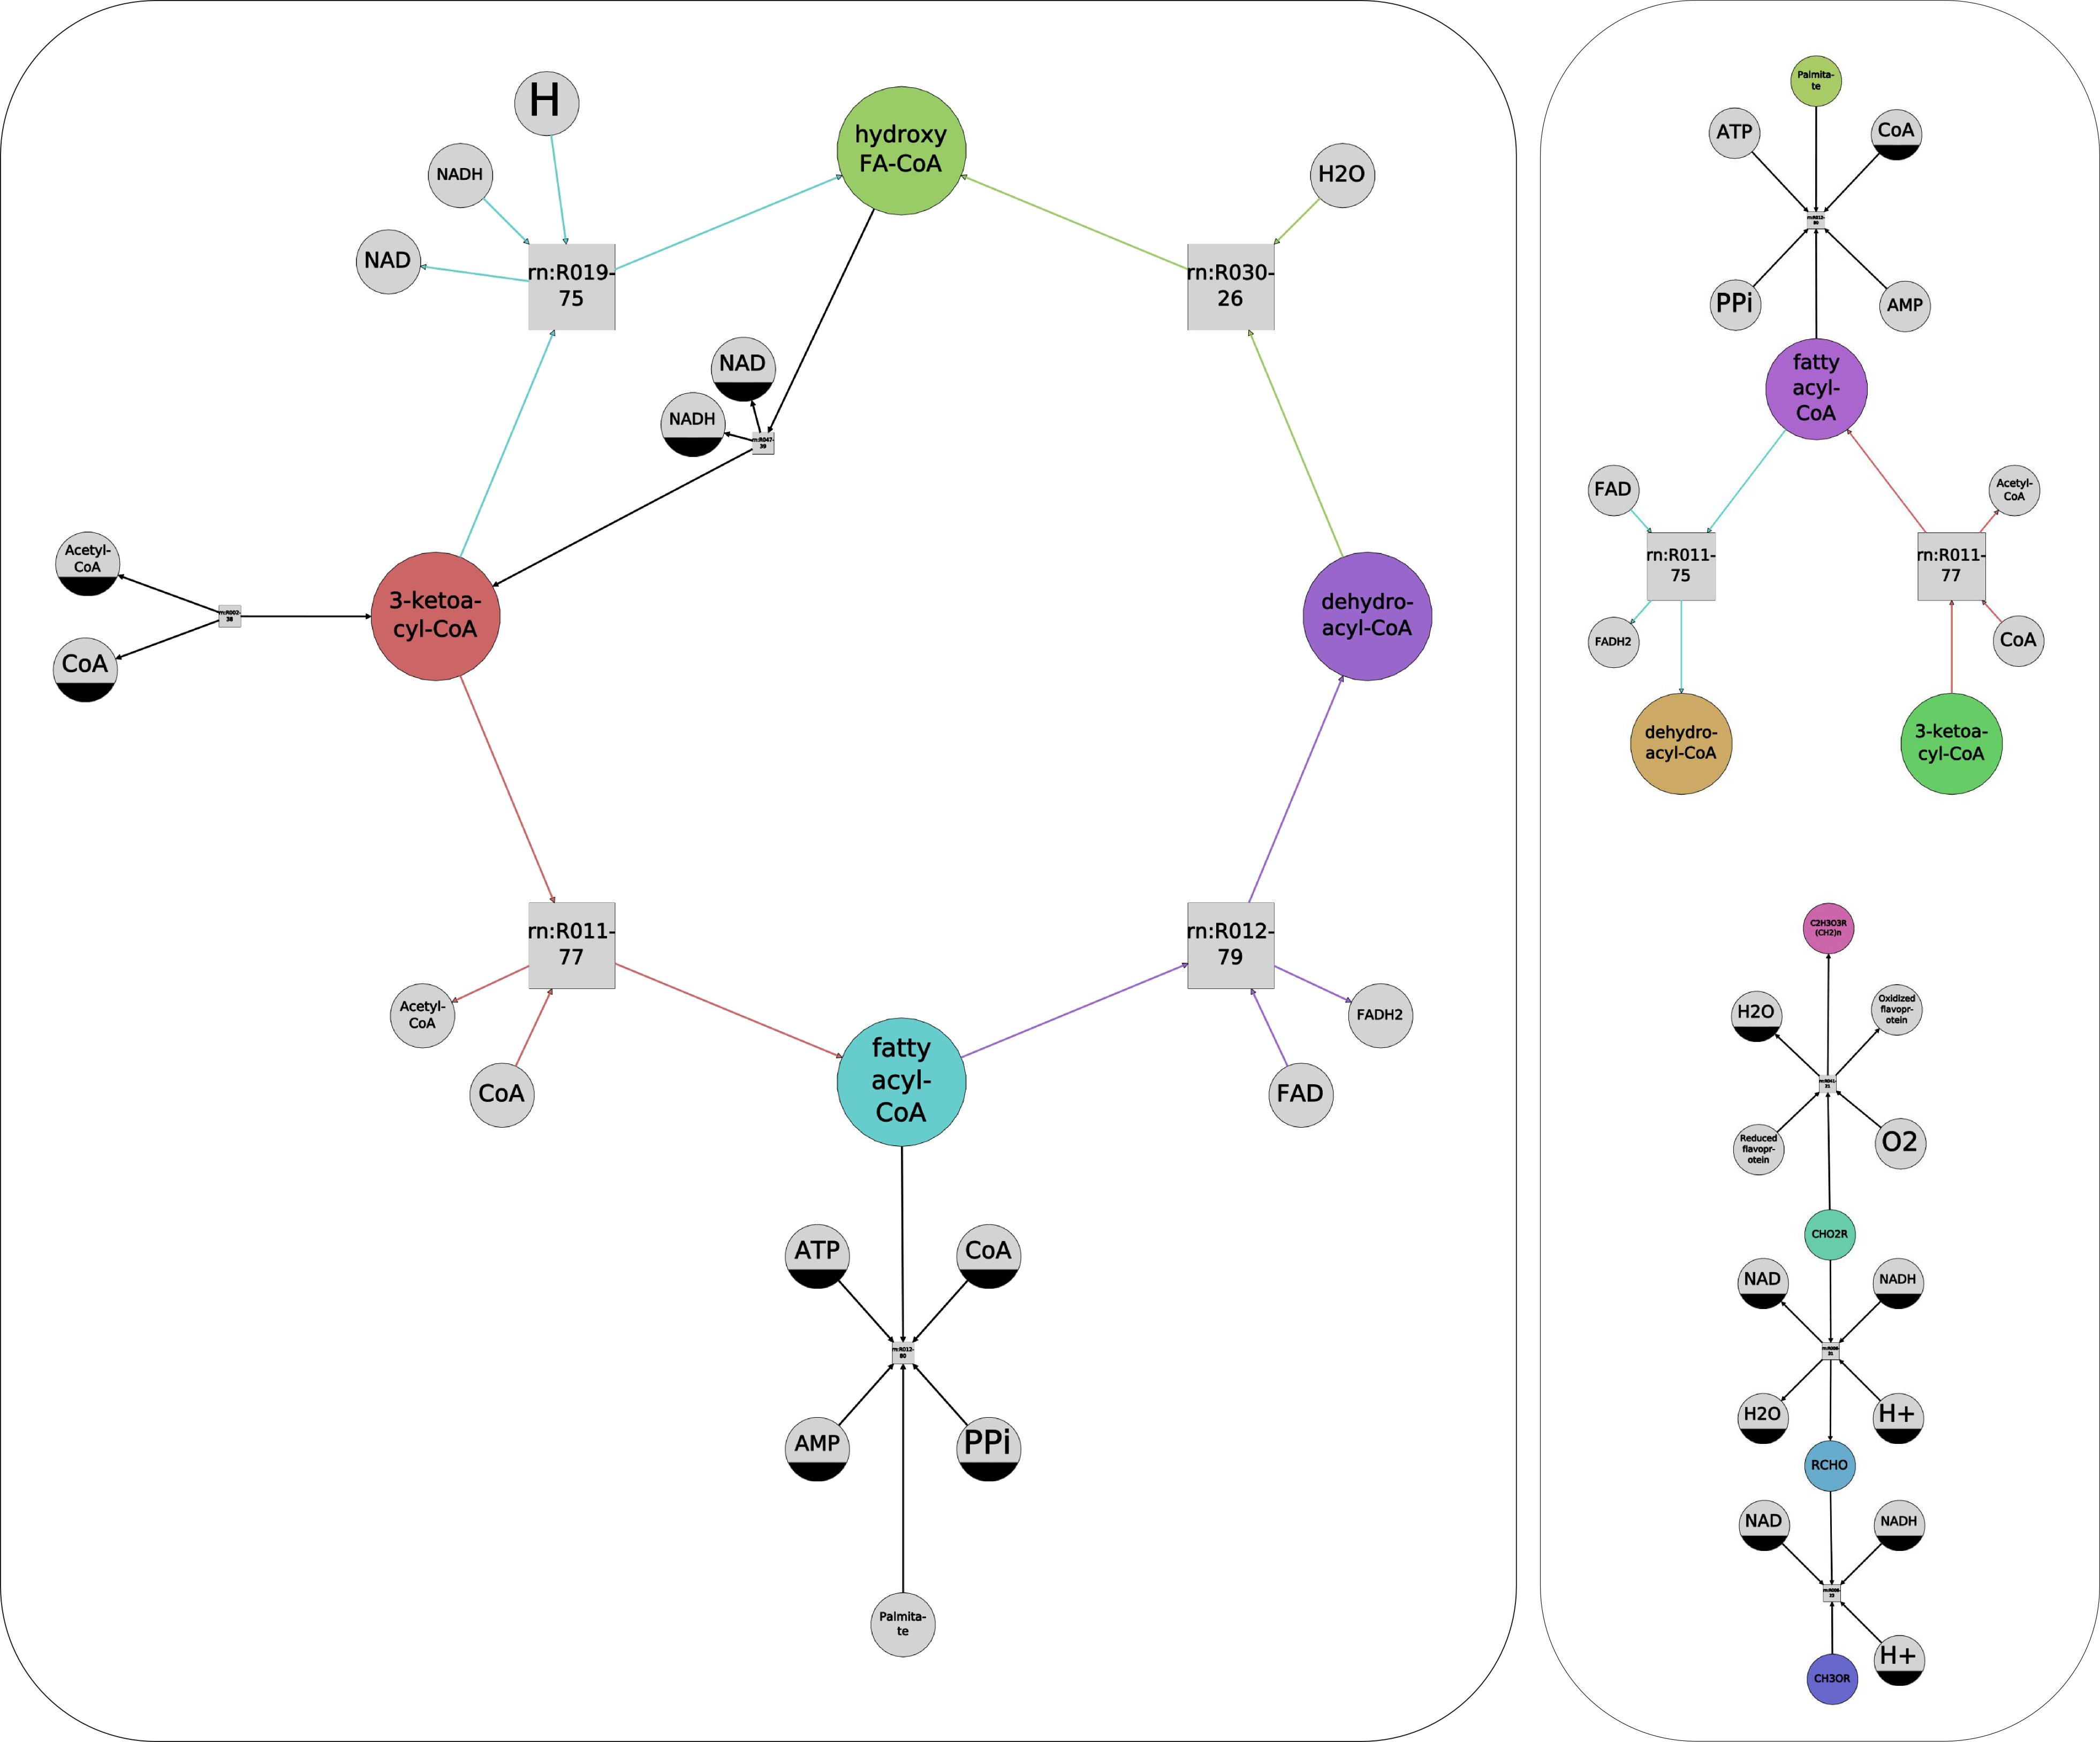
\includegraphics[scale=0.16]{pics/gen.png} 

      The figure shows the generalizations of \textit{Escherichia coli} (left) and \textit{Saccharomyces cerevisiae} (right) fatty acid oxidation models.
      
      (The figure is produced using the Tulip graph visualization tool.)
\caption{Generalization of the \textit{Escherichia coli} and \textit{Saccharomyces cerevisiae} models}
\label{fig:gen}
\end{figure}


\section*{Conclusion}
TODO: We can merge, compare, etc. models using this technique.

\newpage
%\section*{Restrictions}
%
%\nc{The species label generalization should not decrease the number of species (entity pools) participating in a reaction.}
%
%"A species in SBML refers to a pool of entities that (a) are considered indistinguishable from each other for the purposes of the model, (b) may participate in reactions, and (c) are located in a specific compartment." (SBML specification)
%
%"An entity pool is a population of entities that cannot be distinguished from each other, when it comes to the SBGN Process Description Level 1 map. For instance all the molecular entities that fulfill the same role in a given process form an entity pool." (SBGN)
%
%"A reaction in SBML represents any kind of process that can change the quantity of one or more species in a model. <…> At minimum, to describe a reaction in SBML, it is necessary to define its structural properties, specifically the participating reactants and/or products (and their corresponding stoichiometries) and the reversibility of the process" (SBML)
%
%"A process transforms a set of entity pools (represented by EPNs in SBGN Process Description Level 1) into another set of entity pools." (SBGN)
%
%"In a chemical reaction, reactants change into products. A chemical reaction may be represented by a balanced chemical equation, showing the formulae of the reactants and products, and the changes that take place. <...> There are two important facts about any chemical equation: first, all the atoms present in the reactants are also present in the products; and secondly, a balanced chemical reaction shows the number of species taking part in the reaction." (Advanced Chemistry By Michael J. Clugston, Rosalind Flemming  Oxford University Press, Sept 8, 2000 Science) 
%
%\section*{Introduction}
%			
%			Metabolic networks are large systems composed of chemical reactions happening inside a cell. These reactions convert the energy from the environment into the one useful to the organism, and synthesize small molecules that are needed for the organism growth. 
%			
%			There are several formats of metabolic model representation. Examples of ones widely adopted by the community are SBML~\cite{Hucka03} and SBGN~\cite{LeNovere09}. SBML is an XML-like format, describing compartments, chemical species presented in the compartments, and reactions between them. SBGN represents a network as a graph: Species nodes are connected by edges to the nodes of reactions they take part in.
%			
%			Depending on their purpose models can differ in coverage, level of precision, and the information representation. For instance, some models focus on a particular process or pathway happening inside the cell, e.g. \emph{BIOMD0000000219}~\cite{Singh2006} that describes tricarboxylic acid cycle and glyoxylate bypass in \emph{Mycobacterium tuberculosis} in 15 reactions between 13 species.  While some are genome-scale networks covering all the known metabolic reactions in the organism, for instance \emph{MODEL1111190000}~\cite{Loira12} representing a genome-scale network of the yeast \emph{Yarrowia lipolytica}, incorporating 1988 reactions between 2773 species in 17 compartments.
%			
%			The level of precision also differs between models, which answers a practical need: Depending on the purpose of the model, more or less detailed representation is desirable. For example, \textit{$\beta$-oxidation of fatty acids}~\cite{Metzler01} can be described in a model in a more generic way: transforming \textit{Acyl-CoA} into \textit{Enoyl-CoA}, then to \textit{1-3-Hydroxyacyl-CoA}, etc.; or in more details, specifying those reactions for each of the \textit{Acyl-CoA} species presented in the organism cell (e.g. \textit{decanoyl-CoA}, \textit{dodecanoyl-CoA}, etc.). The latter, more precise model, is needed for a simulation, while the more general one is clearer to a human. 
%			
%			Model design principles may also vary between different models. For example, elements of an SBML/SBGN model (species, compartments, reactions) are associated with names. The names can differ from model to model in the choice of a specific synonym, e.g. \textit{lauroyl-CoA} vs \textit{dodecanoyl-CoA} for a species name.
%			
%			All these issues make it hard to compare metabolic models, find common parts, combine and map them. Thus, a way to scale models to the needed levels of precision is desirable. Scaling of the elements of metabolic models can be achieved with the help of ontologies. An ontology is “a~specification of a~conceptualisation"~\cite{Gruber95}, defining a controlled vocabulary in the domain of interest and representing relationships between the terms. The most common relationship is the hierarchical one (\textit{"is\_a"}) between more specific and more general terms. SBML format supports annotation of its elements (i.e. mapping to ontological terms); different tools and libraries for annotation are developed, e.g. libAnnotationSBML~\cite{Swainston09}.
%			
%			An example of an ontology used in metabolic modelling domain is ChEBI~\cite{deMatos10}, which classifies chemical compounds. Associating species names in a metabolic model to ChEBI terms allows for unambiguous names for species, as well as maps together synonymous names, and enriches a model with the knowledge about relationships between its species, e.g. hierarchical ones: \textit{decanoyl-CoA}, \textit{dodecanoyl-CoA} are both descendants of \textit{fatty acyl-CoA}. For classification of enzymes the Gene Ontology~\cite{Ashburner2000} can be used. Situation with the reaction classification is less developed. To our knowledge, there is no ontology classifying broad range of reactions. Rhea database of chemical reactions~\cite{Alcantara2012} can be considered as such, but it covers only few organisms.\nc{TODO: Reactome, MetaCyc, BioPax}
%			
%			In this paper we introduce a method that allows for knowledge-based scaling of metabolic models targeted for desired level of details, thus providing a way to classify models.
%			
%\section*{Model Generalization}
%The model generalization procedure consists of two steps: species label generalization and reaction factoring, and is shown on Figure~\ref{fig:modgen}.
%Species label generalization can be considered as choosing a more general term in the ChEBI ontology and replacing the species label with it. All the species that obtain the same new label are generalized into one. Reactions factoring is based on species label generalization: Reactions transforming the same generalized reactants into the same generalized products are factored together into a generalized reaction.
%
%\begin{figure}
%\includegraphics[scale=1]{../../../pics/spgrf.png} 
%
%      The figure shows species label generalization and reaction factoring operations.
%\caption{Model generalization procedure}
%\label{fig:modgen}
%\end{figure}
%
%
%
%\subsection*{Species Label Generalization}
%The species in the model are divided into two groups: ubiquitous and specific. Ubiquitous species are those participating in many reactions (at least 10, where 10 is an adjustable parameter), such as water, hydrogen, oxygen, etc. They are common for most of the models, thus do not need to be generalized. Specific species are all the others, they are divided into groups of similar species and generalized accordingly.  
%
%To be able to define "similar" species in the model, we introduce the way to compare them.
%
%Def: A relation $\leq$ is a partial order on a set $S$ if it has:
%\begin{itemize}
%\item Reflexivity: $\forall a \in S\:a \leq a$
%\item Antisymmetry: $a \leq b \land b \leq a \implies a=b $
%\item Transitivity: $a \leq b \land b \leq c \implies b \leq c $~\cite{WolframAlpha}
%\end{itemize}
%		An intuitive way to define a partial order $\leq$ on a set $S$ of the ChEBI ontology terms is: $t_{1} \leq t_{2}$ if $t_{1}$ is equal, or a descendant of $t_{2}$ in the ChEBI hierarchy.
%		
%		Depending on the level of generalization needed, each term can be generalized by replacing it with one of its ancestors. It is important though that every two terms have at most one common ancestor at the level chosen for the generalization, which is not the case for ChEBI. For instance, as shown on Figure~\ref{fig:chebi}, \textit{hexadecenoyl-CoA~(CHEBI:24549)} and \textit{trans-2-octadecenoyl-CoA~(CHEBI:50570)} have two closest common ancestors: \textit{unsaturated fatty acyl-CoA~(CHEBI:51006)} and \textit{long-chain fatty acyl-CoA~(CHEBI:33184)}. Both of them are upper bounds, but they are incomparable being on the same level of the ChEBI hierarchy: direct descendants of \textit{fatty acyl-CoA~(CHEBI:37554)}. This causes a problem to the species label generalization by making the choice of the generalized label ambiguous: In order to generalize \textit{hexadecenoyl-CoA} and \textit{trans-2-octadecenoyl-CoA} into one species should we choose \textit{unsaturated fatty acyl-CoA} or \textit{long-chain fatty acyl-CoA}? Or, if both \textit{unsaturated fatty acyl-CoA} and \textit{long-chain fatty acyl-CoA} are to be used in the generalized model, which of their common descendants should be generalized into the first one, and which into the second? 
%		
%\begin{figure}
%
%\includegraphics[scale=1]{../../../pics/chebi.png} 
%
%      The figure shows an example of multiple inheritance in the ChEBI ontology: \textit{hexadecenoyl-CoA} and \textit{trans-2-octadecenoyl-CoA} have two closest common ancestors \textit{unsaturated fatty acyl-CoA} and \textit{long-chain fatty acyl-CoA}.
%\caption{Multiple Inheritance in ChEBI}
%\label{fig:chebi}
%\end{figure}
%
%Moreover, it turns out that using only hierarchical relationships on the ChEBI ontology is not always enough. Examples show, that similar reactions can happen to the acid and the base in a conjugate acid-base pair. A conjugate acid-base pair is two species, one an acid and one a base, that differ from each other through the loss or gain of a proton~\cite{stoker2012general}. For instance, in Rhea reaction database, the acyl-CoA oxidase reaction (RHEA:28354): $\textit{decanoyl-CoA} + \textit{FAD} + \textit{H+} \rightarrow \textit{trans-dec-2-enoyl-CoA} + $\textit{FADH$_2$} is found for both \textit{decanoyl-CoA~(CHEBI:28493)} and its conjugate base \textit{decanoyl-CoA(4-)~(CHEBI:61430)}. Thus, we would like such reactions to be factored into one in the generalized model. To establish a conjugate acid-base pair correspondence in the ChEBI ontology not the hierarchical (\textit{is\_a}) but special \textit{is\_conjugate\_base\_of} and \textit{is\_conjugate\_acid\_of} relationships are used.
%
%Finally, the model itself provides some restrictions. In order to preserve the topology of the reactions in the model: keep the number of different reactants and products, and avoid the appearance of cyclic generalized reactions (having the same generalized species as a reactant and a product), any two species participating in the same reaction must not be generalized into the same species. Figure~\ref{fig:restriction} shows examples of the reaction topology restriction violations.
%
%		
%\begin{figure}
%
%\includegraphics[scale=1]{../../../pics/restriction.png} 
%
%      The upper figure shows the species label generalization that reduces the number of reactants of a reaction.
%      
%      The bottom figure shows the species label generalization that merges a reactant and a product, leading to a cyclic generalized reaction.
%\caption{Reaction Topology Restriction Violations}
%\label{fig:restriction}
%\end{figure}
%
%These reasons justify the need of a more  complex partial order on the set of ChEBI terms, that takes into account both \textit{is\_a} and \textit{is\_conjugate\_base/acid\_of} relationships, makes the choice of the generalized term unique, and satisfies the restriction imposed by the reaction topology in the model.
%
%Def: Terms $t_1$ and $t_2$ are relationship-equivalent $t_1 \tilde{=} t_2$ iff they are equivalent  $t_1 = t_2$ or there exists a chain of \textit{is\_conjugate\_base/acid\_of}  relationships linking them to each other in the ontology.
%
%Def: Term $t$ is a generalized direct descendant/ancestor of a term $T$ iff $t$ or any of its relationship-equivalents is a direct descendant/ancestor of $T$ or of any of its relationship-equivalents.
%
%Def: Term $t$ is a generalized descendant/ancestor of  a term $T$ iff $t$ is a generalized direct descendant/ancestor of $T$ or of any generalized descendant/ancestor of $T$.
%
%Then we can define a new binary relation $\tilde{\leq}$ on a set $S$ of the ChEBI ontology terms as: $t_{1} \tilde{\leq} t_{2}$ if $t_{1}$ is relationship-equal, or a  generalized descendant of $t_{2}$ in the ChEBI hierarchy. This is a partial order on the set $S$ with regard to relationship-equivalence.
%This definition takes into account \textit{is\_conjugate\_base/acid\_of} relationships. But the  prohibition of multiple generalized ancestors and the reaction topology restriction are still not satisfied.
%
%To satisfy them, we will modify the set $S$ itself. First of all, we will remove the terms other than those presented in the model (further addressed as model terms), their ancestors up to the level of generalization (that can be relative, e.g. $\textit{current level} - 3$, or absolute, e.g. ChEBI root \textit{chemical entity} for the most generic model). We will look at the subontology of ChEBI (induced ontology) including those terms and \textit{is\_a} and \textit{is\_conjugate\_base/acid\_of} relationships between them. We will then remove some more terms and relationships from this subontology in order to make it coherent with the restrictions.
%The generalized terms are now to be looked for among the root terms of the induced ontology (maximal elements of the poset).
%
%Def: Two terms $t_1$ and $t_2$ are "similar" with respect to the term $T$ if they are both generalized descendants of $T$, i.e. it is possible to access T from both $t_1$ and $t_2$ by either climbing the hierarchy (going from a more specific term, to a more generic one) and/or by replacing any of the terms on the way with its relationship-equivalent. 
%A set of "similar" terms induced by a term $T$ includes $T$, its relationship-equivalent terms, and their generalized descendants. As the sets of "similar" terms induced by non-roots are included into their ancestors' ones, we will consider only the sets of "similar" terms induced by the root terms. Figure~\ref{fig:similar} shows an example of a set of "similar" terms induced by \textit{medium-chain fatty acyl-CoA}.
%
%\begin{figure}
%
%\includegraphics[scale=1]{../../../pics/sim_gr.png} 
%
%      The green area represents the set of "similar" terms induced by \textit{medium-chain fatty acyl-CoA}, and includes itself, its descendants (\textit{decanoyl-CoA} and \textit{lauroyl-CoA}), and terms connected by \textit{is\_conjugate\_base/acid\_of} relationships (\textit{decanoyl-CoA(4-)} and \textit{lauroyl-CoA(4-)}).
%\caption{Set of "Similar" Terms}
%\label{fig:similar}
%\end{figure}
%
%%We define several simplifications on the induced ontology, illustrated in Figure~\ref{fig:rules}:
%%\begin{itemize}
%%\item If a term $t$ is not a model term, has no descendants and no ancestors,  then $t$ can be removed.
%%\item If a term $t$ is not a model term, neither is each of its relationship-equivalent terms, and none of them have descendants, then $t$ can be removed.
%%\item If a term $t$ is not a model term, has not more than one direct ancestor, no relationship-equivalent terms, and not more than one direct descendant, than it can be removed, moving its direct descendant level up in the hierarchy.
%%\end{itemize}
%%None of those simplifications affect the choice of the maximal element ancestors for model terms.
%%
%%\begin{figure}
%%
%%\includegraphics[scale=1]{../../pics/rules.png} 
%%
%%      The top figure shows the removal of a term $t$ that is not a model term, has no descendants and no ancestors.
%%      
%%      The middle figure shows the removal of a leaf term $t$ that is not a model term and is relationship-equivalent only to a leaf non-model term $t'$.
%%      
%%      The bottom figure shows the removal of a term $t$ that is not a model term, has only one direct descendant  term $\tau$, only one direct ancestor term $T$, and no relationship-equivalent terms.
%%\caption{Ontology Simplification Rules}
%%\label{fig:rules}
%%\end{figure}
%
%We then proceed to the process of satisfying the reaction topology restrictions. 
%First of all, we remove any \textit{is\_conjugate\_base/acid\_of}  relationships between model terms participating in the same reaction. \nc{TODO: Or we do not add those relationships at all in that case. Does not happen in Yali model though.}
%
%Then, all the terms inducing sets of "similar" terms that violate at least one restriction are collected. Those terms are common generalized ancestors of pairs of model terms that participate in the same reaction. For each of such terms $T_i$, if the removal of $T_i$ does not lead to an appearance of a new model term root (consequently of a new one-element-only set of "similar" terms), we remove it. If it does and also $T_i$ is a root itself, we keep it. If it does, but $T_i$ is not a root itself, we raise all its direct descendants one level up in the hierarchy (so that they become direct descendants of all the direct ancestors of $T_i$), and then remove $T_i$. Raising a term in the ChEBI hierarchy does not add a new relationship to the ontology, but only uses the inferred one.
%
%After this, if for any term pair $t_1$, $t_2$ the restriction is still unsatisfied, it means that their common generalized ancestor $T$ is a root term, having at least one direct model term descendant. To satisfy the restriction, we should remove at least one of the terms $t_1$, $t_2$ from the set of "similar" terms induced by $T$, i.e. remove the generalized hierarchical relationship between them.  We choose the term that has more generalized ancestors and relationship-equivalent terms, i.e. is more connected and will belong to a larger set of "similar" terms after the relationship removal. We then remove all the direct \textit{is\_a} relationships between its generalized ancestors or it and $T$.
%
%\begin{figure}
%
%\includegraphics[scale=1]{../../../pics/mod.png} 
%
%      The reaction shown on the bottom left figure poses the restriction that \textit{decanoyl-CoA} and \textit{trans-dec-2-enoyl-CoA} must not belong to the same set of "similar" terms. This restriction is violated for the ontology shown on the top left figure. Model terms are shown in green. To satisfy it, we first of all look for the common ancestors of the two terms (shown in red). They are \textit{medium-chain fatty acyl-CoA} and \textit{fatty acyl-CoA}. The removal of \textit{fatty acyl-CoA} would lead to appearance of a new model term root (\textit{tetracosanoyl-CoA}), thus we keep it. \textit{Medium-chain fatty acyl-CoA} is not a root, thus we remove it and raise its direct descendants one level up in the hierarchy, as shown on the top right figure. The restriction is still unsatisfied, as the common ancestor \textit{fatty acyl-CoA} still belongs to the ontology. We choose \textit{trans-dec-2-enoyl-CoA} as it is connected to more other terms than \textit{decanoyl-CoA}, and remove all the direct \textit{is\_a} relationships between its generalized ancestors (\textit{saturated fatty acyl-CoA}) or it and \textit{fatty acyl-CoA} (shown in light red). The resulting ontology represented on the bottom right figure satisfies the restriction.
%\caption{Ontology Modifications}
%\label{fig:mod}
%\end{figure}
%
%These steps are shown on Figure~\ref{fig:mod}. We repeat them until all the restrictions are satisfied. At each iteration at least one relationship is removed, making the subontology less connected, thus the process terminates.
%
%The resulting ontology is a subgraph of ChEBI with the inferred hierarchical relationships (i.e. any term $\tau$ that \textit{is\_a} indirect descendant of a term $t$,  also \textit{is\_a}  $t$). In the resulting ontology, all the reaction topology restrictions are satisfied. 
%
%The last step is to satisfy the multiple generalized root ancestor prohibition. Each model term belongs to at least one set of "similar" terms induced by roots. If it belongs to several ones, then one should be chosen out of them to be used for the species label generalization, while all the direct \textit{is\_a} relationships between the model term's generalized ancestors and the other roots should be removed. The root terms being the only generalized root ancestors for at least one model term are primary, the others are secondary. In case of a multiple choice of a generalized root ancestor for a model term, the primary ones are prioritised, as being supported by at least one more model term. If there are no or several primary generalized root ancestors for a model term, the one inducing the smallest set of "similar" terms is chosen as being the most precise one. 
%
%\nc{Actually, we could look back at the model and choose the generalized ancestor that does not add new connectivity: does not connect two generalized reactions, such that there was no specific species, that would connect the reaction prototypes in the original model (future work). But on the other hand, if the precision level is specified by the user, then he or she might want this extra-connectivity to be added, or at least does not want to distinguish between those species...}
%
%After all those steps, the resulting induced ontology defines in a unique way the partition of the set of model terms into non-intersecting subsets of "similar" terms. This partition is used to generalize species labels in the model.
%
%\subsection*{Reaction Factoring}
%After the species labels are generalized, each reaction $r$ in the model is associated to the two-part key: $(R, P)$, where $R = (s_{r_1}, ...,  s_{r_n})$ and $P = (s_{p_1}, ..., s_{p_m})$ are sorted lists of generalized reactants and generalized products of $r$ accordingly. If $r$ is reversible and $P$ is less than $R$, the key is replaced with the one for the reversed reaction: $(P, R)$. 
%Reactions associated to the same key are factored into one generalized reaction. 
%
%\section*{Model Hierarchy}
%
%			Having defined a partial order on the set of ChEBI terms, we can define it also on the set of SBML metabolic models annotated with ChEBI. 
%For two models $M_1, M_2$ $M_1 \leq M_2$ if there exists a subontology of ChEBI defining a species label generalization procedure $g$ mapping each of the species of $M_1$ to a species of $M_2$ such that for every reaction $r: s_{r_1} + ... + s_{r_n} \rightarrow s_{p_1} + ... + s_{p_m}$ in the model $M_1$ there exists a reaction $\breve{r}$ in the model $M_2$ between the corresponding generalized species: $\breve{r}: g(s_{r_1}) + ... + g(s_{r_n}) \rightarrow g(s_{p_1}) + ... + g(s_{p_m})$. 
%
%\section*{Model Specialization}
%Model specialization is an inverse process to the model generalization, and requires a subontology of ChEBI defining the descendants for the terms to be specialized. 
%For each reaction in the model, we consider all possible specializations and search for them in reaction databases (Reactome, MetaCyc, BioPax, Rhea). Those of the reactions that exist in databases, are added to the specified model. Reaction specializations are obtained from the given reaction by replacing each of the participants found in the ChEBI subontology by any of its descendants.
%Model specialization is shown on Figure~\ref{fig:specif}.
%
%
%\begin{figure}
%
%\includegraphics[scale=1]{../../../pics/specif.png} 
%
%      Model specialization consists of two steps: expanding terms using a given ontology, and choosing those of possible reactions that exist in a reaction database.
%\caption{Model Specialization}
%\label{fig:specif}
%\end{figure}
%							
%							
%							
%\section*{Applications}
%\begin{itemize}
%\item understand
%\item visualize
%\item compare
%\item merge
%\item identify pathways
%\item use as a scaffold
%\end{itemize}
%
%\section*{Use cases}
%\nc{
%High-level understanding of reaction networks is informative. Verification: if the higher level is crazy, then there is a problem with inferencing. 
%
%Take a well-known model, say e.coli, loss/gain/alternative pathway.
%
%Make a mistake in a model => easy to find.}
%
%We will look at fatty acid metabolism pathways in several models: a genome-scale model of an yeast \textit{Yarrowia lipolytica}, and two path2model~\cite{???} pathways: fatty acid metabolism of a bacteria \textit{Escherichia coli} and an yeast \textit{Saccharomyces cerevisiae}. We will generalise all the three models, and compare results and induced ChEBI ontologies for them. 
%
%In \textit{Yarrowia lypolitica} fatty acid oxidation is happening in the peroxisome compartment, so we have extracted a submodel of the initial model, including only those species and reactions, that are happening in the peroxisome. This submodel as attached as additional file~1. 
%
%
%
%
%
%
%	\section*{Discussion}
%		Generalization as rules: given an ontology and a population of models, 
%we can define a most informative set of graph rewriting rules
%
%Simplified model is easier to visualize.
%
%		Possible to the community to impose levels of abstraction: ChEBI slims as GO slims
%		
%		"isa" reaction - another approach
%			
%







%%%%%%%%%%%%%%%%%%%%%%%%%%%%%%%%%%%%%%%%%%%%%%%%%%%%%%%%%%%%%
%%                  The Bibliography                       %%
%%                                                         %%              
%%  Bmc_article.bst  will be used to                       %%
%%  create a .BBL file for submission, which includes      %%
%%  XML structured for BMC.                                %%
%%  After submission of the .TEX file,                     %%
%%  you will be prompted to submit your .BBL file.         %%
%%                                                         %%
%%                                                         %%
%%  Note that the displayed Bibliography will not          %% 
%%  necessarily be rendered by Latex exactly as specified  %%
%%  in the online Instructions for Authors.                %% 
%%                                                         %%
%%%%%%%%%%%%%%%%%%%%%%%%%%%%%%%%%%%%%%%%%%%%%%%%%%%%%%%%%%%%%

\newpage
{\ifthenelse{\boolean{publ}}{\footnotesize}{\small}
 \bibliographystyle{bmc_article}  % Style BST file
  \bibliography{db}
 }     % Bibliography file (usually '*.bib' ) 

%%%%%%%%%%%

\ifthenelse{\boolean{publ}}{\end{multicols}}{}


\end{bmcformat}
\end{document}







